\documentclass{article}
\usepackage{iclr2027_conference,times}
\input{math_commands.tex}
\usepackage{amsmath,amssymb,booktabs,graphicx,hyperref,url}
\hypersetup{hidelinks}

\title{Cross-Depth Fixed-Readout Compatibility: Direct Reuse, Restricted Recalibration, and Three-Model Heterogeneity}
\author{}

\begin{document}
\maketitle

\begin{abstract}
Layerwise decodability does not establish that the same decision rule remains usable across depths; direct readout reuse is therefore a distinct empirical question. We study this question with a version-controlled registered source-target protocol: a task readout is fit at one decoder depth, reused without retraining at every target depth, and compared with a deliberately restricted FIT-only calibration diagnostic. Across Qwen3-1.7B, OLMo-2-1B-Instruct, and Meta-Llama-3.2-1B-Instruct, normalized depth distance is positively associated with degradation under the fixed readout. The models nevertheless show different source/target organization and restricted-recalibration endpoints. Qwen is target-dominant with unsupported registered LOW-D recovery, OLMo is source-dominant with supported LOW-D recovery, and Llama is target-dominant with supported LOW-D recovery. Complementary-split non-replication and an unsupported registered degradation-based predictor further limit a uniform recovery account. A post-closure similarity comparison provides secondary descriptive context, not a replacement for the directed analysis. We report a bounded three-model characterization of operational compatibility and heterogeneity, limited to the tested models, carrier, task panel, and registered conditions.
\end{abstract}

\section{Introduction}
Layerwise probing asks whether a task is decodable at each depth. That question does not establish that the same decision rule remains usable across depths; direct readout reuse is therefore a distinct empirical question. A layer may support a separately fitted decoder while a fixed decoder from another depth fails, and limited recalibration may recover utility after direct reuse fails. This matters for interpreting cross-layer probes, monitoring and readout portability, and representation comparison without silently conflating different operational tests.

This paper asks: when a task readout is fit at one decoder depth and applied without retraining at another, how do direct operational compatibility, degradation, and restricted FIT-only recovery vary across depth and across three tested language models? We answer this question with full directed source-target matrices. \texttt{C0}, \texttt{D}, and \texttt{R} are transparent operational bookkeeping quantities for direct reuse, source-relative degradation, and gain under the registered restricted calibration; none is presented as an individually novel metric. Direct reuse and restricted recoverability answer different operational questions; reporting only one can hide the distinction between immediate readout portability and limited recalibratability.

All three models show positive distance-associated degradation, but the source/target organization and restricted-recalibration endpoints do not collapse into one common ordering. Qwen is target-dominant with unsupported LOW-D recovery; OLMo is source-dominant with supported LOW-D recovery; Llama is target-dominant with supported LOW-D recovery. Qwen and OLMo happened to align in the initial two-model comparison. A third model was routed prospectively before its result was exposed because two contrasting profiles were insufficient to determine whether the initial descriptive association between source/target organization and LOW-D recovery would persist. Llama's exact profile was not predicted in advance, and the interpretation that it breaks the initial mapping is bounded post-hoc synthesis.

We make three contributions. (1) We establish a controlled direct-reuse / restricted-recalibration contrast under one source-family-disjoint held-out protocol, separating unchanged fixed-readout portability from one deliberately capacity-limited FIT-only calibration diagnostic. (2) We provide a complete cross-depth operational characterization over the registered directed source-target grid in three decoder-only model families, summarizing direct degradation and source/target organization without treating the matrix form itself as new. (3) We provide a three-model joint result with registered boundary evidence: shared distance-associated degradation coexists with different source/target organization and restricted-recalibration endpoint states, while registered non-replication, failed scalar predictors, and prospective third-model routing bound simpler uniform accounts. The resulting question is deliberately narrower than a theory of representation: it concerns the behavior of a specified readout under specified carrier, panel, and conditions.

The novelty claim is not attached to frozen-probe transfer, simple recalibration, readout-performance differences, or directed matrices individually. Prior work establishes these ingredients or closely related operations separately. The contribution here is the controlled separation of unchanged direct reuse from deliberately restricted FIT-only recalibration under one common held-out source-target protocol, together with the resulting three-model joint characterization and registered boundary evidence.

\section{Related Work}
\subsection{Layerwise probing and readout transfer}
Layerwise probing asks what is decodable at different depths. Tuned Lens fits layer-specific affine readouts for intermediate predictions \citep{belrose2023tunedlens}. This paper does not claim novelty for layer-specific readouts. Its measurement holds a source readout fixed during direct transfer and contrasts that direct reuse with one restricted FIT-only calibration diagnostic. The question is operational reuse, not the best decoder available at each layer.

Recent representation-readout decompositions study training dynamics, model-merging failure, or representation/readout interfaces \citep{chou2026twospeeds,janati2026postgrokking,freshhead2025localising,anthes2023diagnosing}. These works establish general prior art for separating representation and readout contributions. This paper asks a different within-model question: holding a source-depth task readout fixed, how does direct cross-depth reuse differ from one registered restricted FIT-only recalibration?

\subsection{Logit-based inspection and activation transfer}
Logit Lens-style inspection exposes predictions through intermediate states \citep{nostalgebraist2020logitlens}. Patchscopes provides a broader framework for inspecting and intervening on hidden representations \citep{ghandeharioun2024patchscopes}. These approaches motivate careful separation of measurement from interpretation, but this paper does not claim novelty for hidden-state inspection or intervention. The present unit is a fixed task readout evaluated across source and target depths.

\subsection{Stitching, alignment, and representation matching}
Model stitching and representation matching study compatibility through learned maps, correspondence procedures, or similarity criteria \citep{bansal2021revisiting,csiszarik2021similarity,maiorca2023latent}. This paper does not introduce a general alignment method or adapter. Smith et al. specifically caution that functional or stitching success does not establish representation equivalence \citep{smith2025functional}. Anthes et al. decompose continual-learning performance loss into representation/readout misalignment and information-loss components using diagnostic readouts and alignment analyses; this establishes general prior art for distinguishing native-readout failure from information loss \citep{anthes2023diagnosing}. Our question is a different within-model cross-depth comparison using one fixed source task interface and one restricted FIT-only calibration branch. The Fresh-Head work is used for representation/readout failure localization in model merging \citep{freshhead2025localising}. Kniazev and Fijalkow train probes at source layers and evaluate them at other layers without retraining, yielding explicit cross-layer transfer matrices \citep{kniazev2026structured}; frozen cross-layer probe transfer and its matrix representation are therefore prior art. Gilg et al. likewise report cross-layer transfer of a probe trained at one layer in the context of persona-dependent preferences \citep{gilg2026probing}. The present contribution is not those operations individually, but their controlled contrast with restricted recalibration under a common held-out protocol.

\subsection{Similarity measures and layerwise progression}
Representation-similarity measures and studies of layerwise progression offer complementary views of hidden-state change \citep{csiszarik2021similarity,jiang2024tracing}. Centered kernel alignment (CKA) was introduced as a representation-similarity measure by Kornblith et al. \citep{kornblith2019similarity}. This paper includes centered linear CKA only as a post-closure secondary comparison. It is not used to define \texttt{C0}, \texttt{D}, or \texttt{R}, and its symmetry means that it does not replace a directed source-target analysis. CKA is not a contribution of this study.

\subsection{Readout and representation boundaries}
SemRF addresses cross-depth comparability by constructing anchor-based semantic reference frames and deriving synchronization, admissibility, and distortion conditions \citep{semrf2026semantic}. The present study does not construct a semantic frame or trajectory geometry. Instead, it measures whether an unchanged supervised task readout remains operationally portable across depth and how one deliberately restricted FIT-only recalibration changes that measurement. ICR Probe studies cross-layer hidden-state dynamics for hallucination detection \citep{icrprobe2025tracking}. These are relevant neighbors, not the present operational decomposition.

\section{Methods}
\subsection{Models, task panel, and carrier}
The panel contains three decoder-only language models. Qwen3-1.7B and OLMo-2-1B-Instruct use the registered model revisions; Llama uses the registered converted-model snapshot authority. The frozen panel contains 1,760 records from 880 source families, four task classes (\texttt{logic}, \texttt{causality}, \texttt{analogy}, and \texttt{definition}), and ten registered surface conditions. FIT, DIAGNOSTIC, and EVAL partitions are source-family disjoint. Exact dataset identities, model revisions, and hashes are provided in the anonymous artifact package.

The registered conditions vary lexical realization, syntactic structure, compression/elaboration, relation explicitness, formal/informal register, a neutral distractor prefix, and anaphoric reference while retaining the registered semantic-class identity.

The carrier is the last valid token at decoder block output: the post-block residual stream before model-level final normalization. The final normalized state and language-model head are excluded. This is the registered carrier, not a claim about the whole representation or its meaning.

\subsection{Source and target depths}
For a model with $L$ decoder blocks, source and target indices range over $0,\ldots,L-1$. Normalized depth is $d(l)=l/(L-1)$. Matrix row $i$ is the source readout depth and column $j$ is the target representation depth. Diagonal entries are source self conditions; off-diagonal entries are direct cross-depth reuse. Normalized depth is an operational indexing convention for within-model source-target summaries; equal normalized depth across models is not assumed to imply functional, semantic, architectural, or representational homology.

\subsection{Fixed reference readout and direct reuse}
Let $X_l$ be the carrier matrix at depth $l$ and $Y$ the task labels. A source readout is fit on FIT data,
\[
 W_s=f(X_s^{\mathrm{FIT}},Y^{\mathrm{FIT}}),
\]
The classifier is multinomial \texttt{LogisticRegression} with \texttt{solver=lbfgs}, \texttt{penalty=l2}, $C=1.0$, \texttt{fit\_intercept=true}, \texttt{tol=1e-4}, \texttt{class\_weight=None}, \texttt{dual=false}, \texttt{max\_iter=1000}, and \texttt{warm\_start=false}. It is fit once at source depth $s$. The same readout is then evaluated on every target depth $t$ using EVAL data. No target-specific refit is part of direct compatibility.

The restricted calibration uses featurewise \texttt{StandardScaler(with\_mean=true, with\_std=true)} statistics estimated from the registered target-depth FIT representations for each condition and retains the registered reference classifier. It is not zero-shot transfer: target-depth FIT representations may estimate the permitted featurewise statistics, but EVAL labels and outcomes cannot affect the fixed source readout, calibration parameters, or pair-selection rule. It is one deliberately limited operator; stronger calibration would answer a different question.

\subsection{Operational quantities}
\texttt{C0}$(s,t)$ is the balanced accuracy of the readout fit at source depth $s$ when evaluated on the target representation at $t$. It is an operational score on the registered task panel. With $C_{\mathrm{self}}(s)=\texttt{C0}(s,s)$, direct degradation is
\[
D(s,t)=C_{\mathrm{self}}(s)-\texttt{C0}(s,t).
\]
\texttt{D} is a readout-relative performance difference. It is not a claim that a signal has disappeared or that a layer has a particular internal function. If $C_{\mathrm{cal}}(s,t)$ is the calibrated target score, restricted recovery is
\[
R(s,t)=C_{\mathrm{cal}}(s,t)-\texttt{C0}(s,t).
\]
\texttt{R} is an absolute gain under the registered restricted FIT-only calibration. We interpret it as restricted recalibratability under this operator, not as general recoverability, equivalence, or preservation.

For off-diagonal pairs we associate $D$ with absolute normalized depth distance $\Delta(s,t)=|d(s)-d(t)|$ using Spearman rank association with average ranks for ties. The source/target dominance index is
\[
 SDI=\frac{V_{\mathrm{source}}-V_{\mathrm{target}}}{V_{\mathrm{source}}+V_{\mathrm{target}}},
\]
where the components are population variances (\texttt{ddof=0}) of off-diagonal row and column means. SDI is a registered scalar summary of source-versus-target organization in the measured matrix.

Registered support is determined by the relevant one-sided 95\% bound: the 5th percentile for positive support and the 95th percentile for negative support. The displayed bracket reports both the 5th and 95th percentiles, rather than a conventional two-sided 95\% confidence interval.

LOW-D means \textbf{low-degradation recovery diagnostic}. It is conditional: the registered mask selects eligible off-diagonal pairs with $D^{\mathrm{DIAG}}(s,t)\leq0$ from DIAGNOSTIC data, and the mean EVAL $\overline R$ is then measured on that frozen set. DIAG denotes the DIAGNOSTIC split and does not denote a matrix diagonal. The selected entries remain off-diagonal source-target entries. The DIAGNOSTIC mask is not re-estimated from EVAL, and EVAL outcomes do not determine membership. LOW-D is not low-dimensional analysis, general recoverability, normalized recovery capacity, an intrinsic model trait, or an operator-independent construct. Its support label applies only to the registered endpoint.

The distance statistic is computed from registered off-diagonal matrix entries; uncertainty is obtained by condition-stratified resampling of EVAL source-family clusters. The bootstrap quantifies source-family sampling uncertainty conditional on the tested model and registered layer grid; it is not population inference over neural-network layers or model architectures. The bootstrap uses 5,000 replicates and \texttt{PCG64(20260819)}. Pairs are not IID inferential units and models are not pooled. A third model was routed prospectively because two contrasting profiles were insufficient to determine whether the initial descriptive association between source/target organization and LOW-D recovery would persist. Llama's exact profile was not predicted before exposure; the mapping-break interpretation is bounded post-hoc synthesis.

\subsection{Prospective third-model routing and statistical rules}
Qwen and OLMo results were already available when the initial descriptive comparison was formed. Their properties happened to align in that initial two-model comparison. A third model was routed prospectively because two contrasting profiles were insufficient to determine whether the initial descriptive association between source/target organization and LOW-D recovery would persist in another tested model. Llama's exact profile was not predicted before exposure. The interpretation that it breaks the simple two-model mapping is a bounded post-hoc synthesis.

Uncertainty is obtained by condition-stratified resampling of EVAL source-family clusters, recomputing the relevant matrix quantity inside each replicate. No row-wise or cell-wise bootstrap is used, and models are not pooled for inference. The LOW-D mask remains the frozen DIAGNOSTIC mask $D^{\mathrm{DIAG}}(s,t)\leq0$ throughout EVAL summarization. Detailed split and condition specifications are in the supplement and version-controlled protocol artifacts.

\subsection{Reproducibility pointer}
Competent reproduction requires the model identities and revisions above, the post-block pre-final-normalization last-valid-token carrier, zero-based source/target indexing, \texttt{LogisticRegression} and \texttt{StandardScaler} settings, the source-family-disjoint FIT/DIAGNOSTIC/EVAL split, registered \texttt{C0}, \texttt{D}, and \texttt{R} definitions, the $D^{\mathrm{DIAG}}(s,t)\leq0$ LOW-D mask, normalized depth $l/(L-1)$, and the source-family condition-stratified cluster bootstrap with 5,000 replicates and \texttt{PCG64(20260819)}. Exact paths and hashes are provided in the anonymous artifact package and version-controlled protocol artifacts. The CKA asset authority records 640 ordered EVAL samples with sample-order hash \texttt{6ff5adb902c7bc691b078c73b3b267005fe37f74b6fd675ba1225d4f8971baea}.

\subsection{Registered execution boundaries}
The split is applied at the source-family level so that related surface conditions do not cross FIT, DIAGNOSTIC, and EVAL boundaries. The source readout is fitted using FIT labels and carrier values only. For direct reuse, the fitted coefficients and class ordering are held fixed while the target carrier is evaluated. The calibration branch estimates only the registered featurewise scaling quantities on FIT data before applying them to target and EVAL data. A target score cannot change the source readout, calibration parameters, or pair-selection rule.

Each condition is retained as a registered measurement rather than selected for a favorable outcome. Condition-pooled quantities use the specified equal-weight aggregation. The full matrix retains diagonal source self conditions and off-diagonal source-target pairs, while the distance statistic is computed only from the registered off-diagonal matrix entries. LOW-D selection is made once from DIAGNOSTIC $D^{\mathrm{DIAG}}(s,t)\leq0$ values and held fixed when EVAL recovery is summarized. The resulting support label is determined by the registered point estimate and one-sided cluster-bootstrap rule; it is not a claim about all possible calibration procedures.

\section{Results}
\subsection{Distance-associated degradation}
All three tested models meet the registered positive-support rule; rounded values and bootstrap bounds are reported in Table 1.
\begin{table}[t]
\centering
\caption{Registered three-model profile values. Values are rounded; exact values are in Supplement S6.}
\label{tab:profile}
\resizebox{\linewidth}{!}{%
\begin{tabular}{lrrrrrrrrrr}
\toprule
Model & Dist. & Dist. 5\% & Dist. 95\% & SDI & SDI 5\% & SDI 95\% & LOW-D mean & LOW-D 5\% & LOW-D 95\% & $n$ / $R^+$ / status\\
\midrule
Qwen3-1.7B & 0.705 & 0.685 & 0.708 & -0.174 & -0.189 & -0.158 & 0.00014 & -0.00010 & 0.00036 & 202 / 0.074 / NOT\_SUPPORTED\\
OLMo-2-1B & 0.752 & 0.744 & 0.758 & 0.525 & 0.491 & 0.558 & 0.04786 & 0.04403 & 0.05152 & 35 / 0.829 / SUPPORTED\\
Llama-3.2-1B & 0.608 & 0.595 & 0.615 & -0.414 & -0.434 & -0.392 & 0.00140 & 0.00073 & 0.00219 & 49 / 0.327 / SUPPORTED\\
\bottomrule
\end{tabular}}
\end{table}

\begin{figure}[t]
\centering
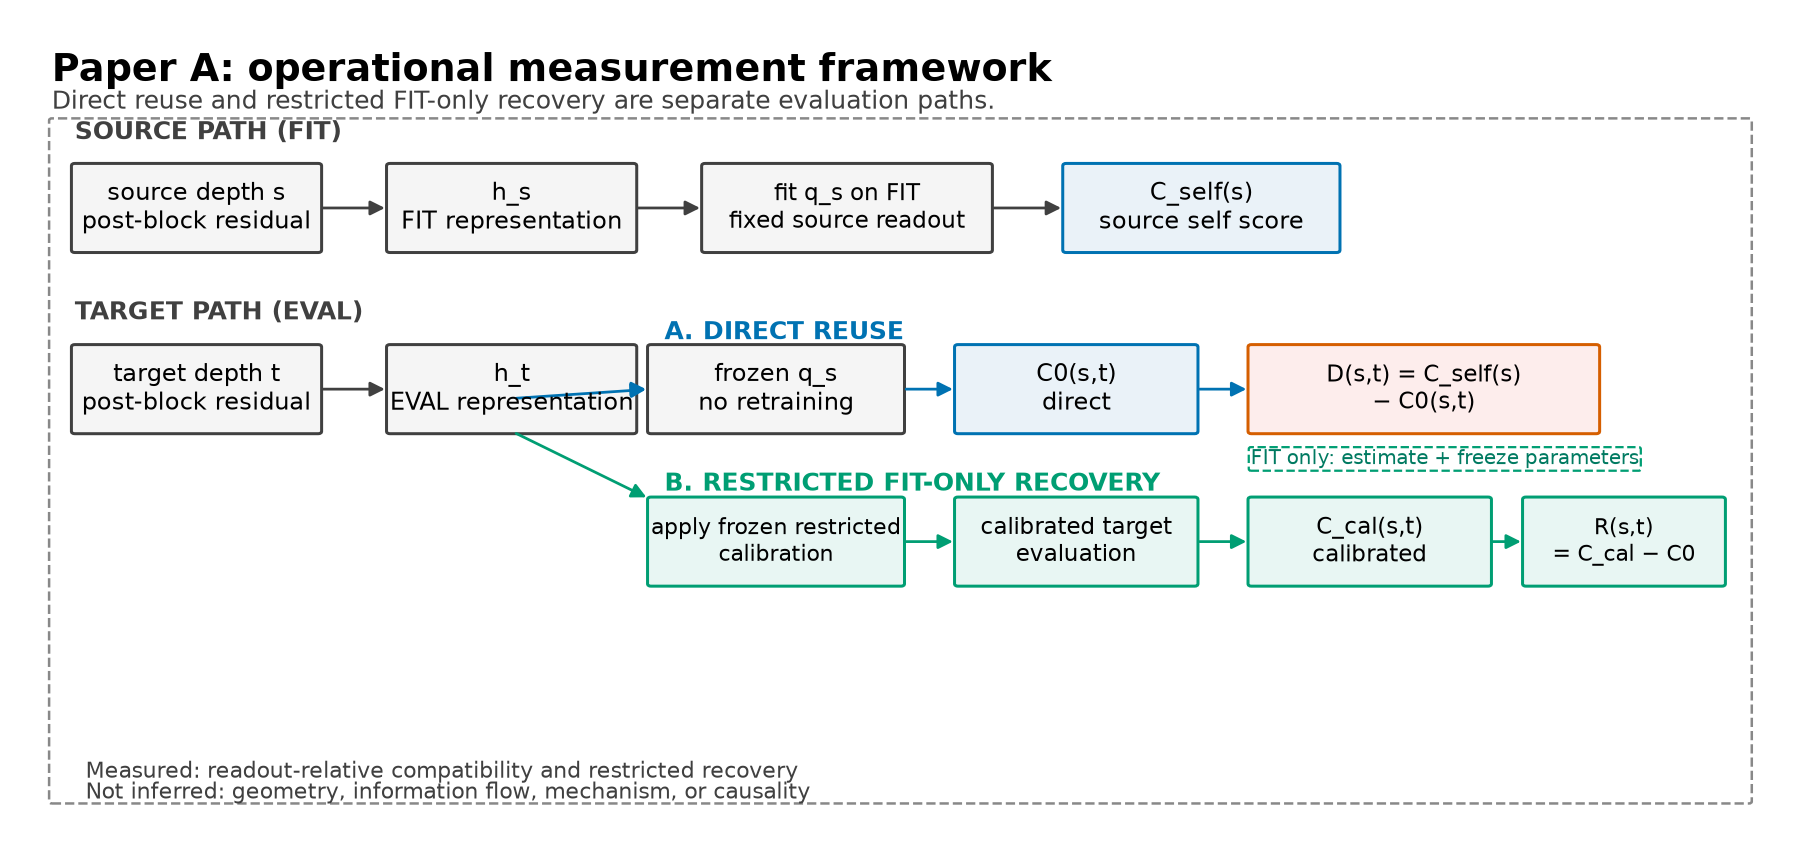
\includegraphics[width=\linewidth]{fig01.png}
\caption{A FIT-trained source readout is evaluated on the source self representation and reused at every target depth. The separate restricted calibration branch is FIT-only. This is a measurement schematic, not a claim about geometry, mechanism, causality, or semantic equivalence.}
\label{fig:framework}
\end{figure}

\subsection{Registered negative evidence}
\begingroup\catcode95=12
EXP-023 was the registered complementary-split replication of the restricted-recovery question. Restricted recalibration did not replicate uniformly across the two splits; the registered cross-split outcome is \texttt{NO\_REPLICATION}. This is evidence of split heterogeneity, not evidence that recovery is absent in every setting.

EXP-024 tested whether a diagnostic degradation magnitude would rank later calibration benefit. Its registered result was \texttt{NOT\_SUPPORTED}, with $\rho=0.284$, $p=0.212$. EXP-025 repeated the panel on OLMo-2-1B-Instruct; degradation was unsupported while restricted recovery was supported, indicating cross-model heterogeneity in the degradation/recovery profile, while its separate predictor remained unsupported ($\rho=0.377$, $p=0.140$). Exact values and split details remain in the supplement.

The lack of uniform recovery across complementary splits and the unsupported degradation-based predictor motivated the shift to full directed matrices and model-profile characterization. The epistemic role of these negative results is preserved while procedural history is compressed.
\endgroup

\subsection{Source/target organization}
\begin{figure}[t]
\centering
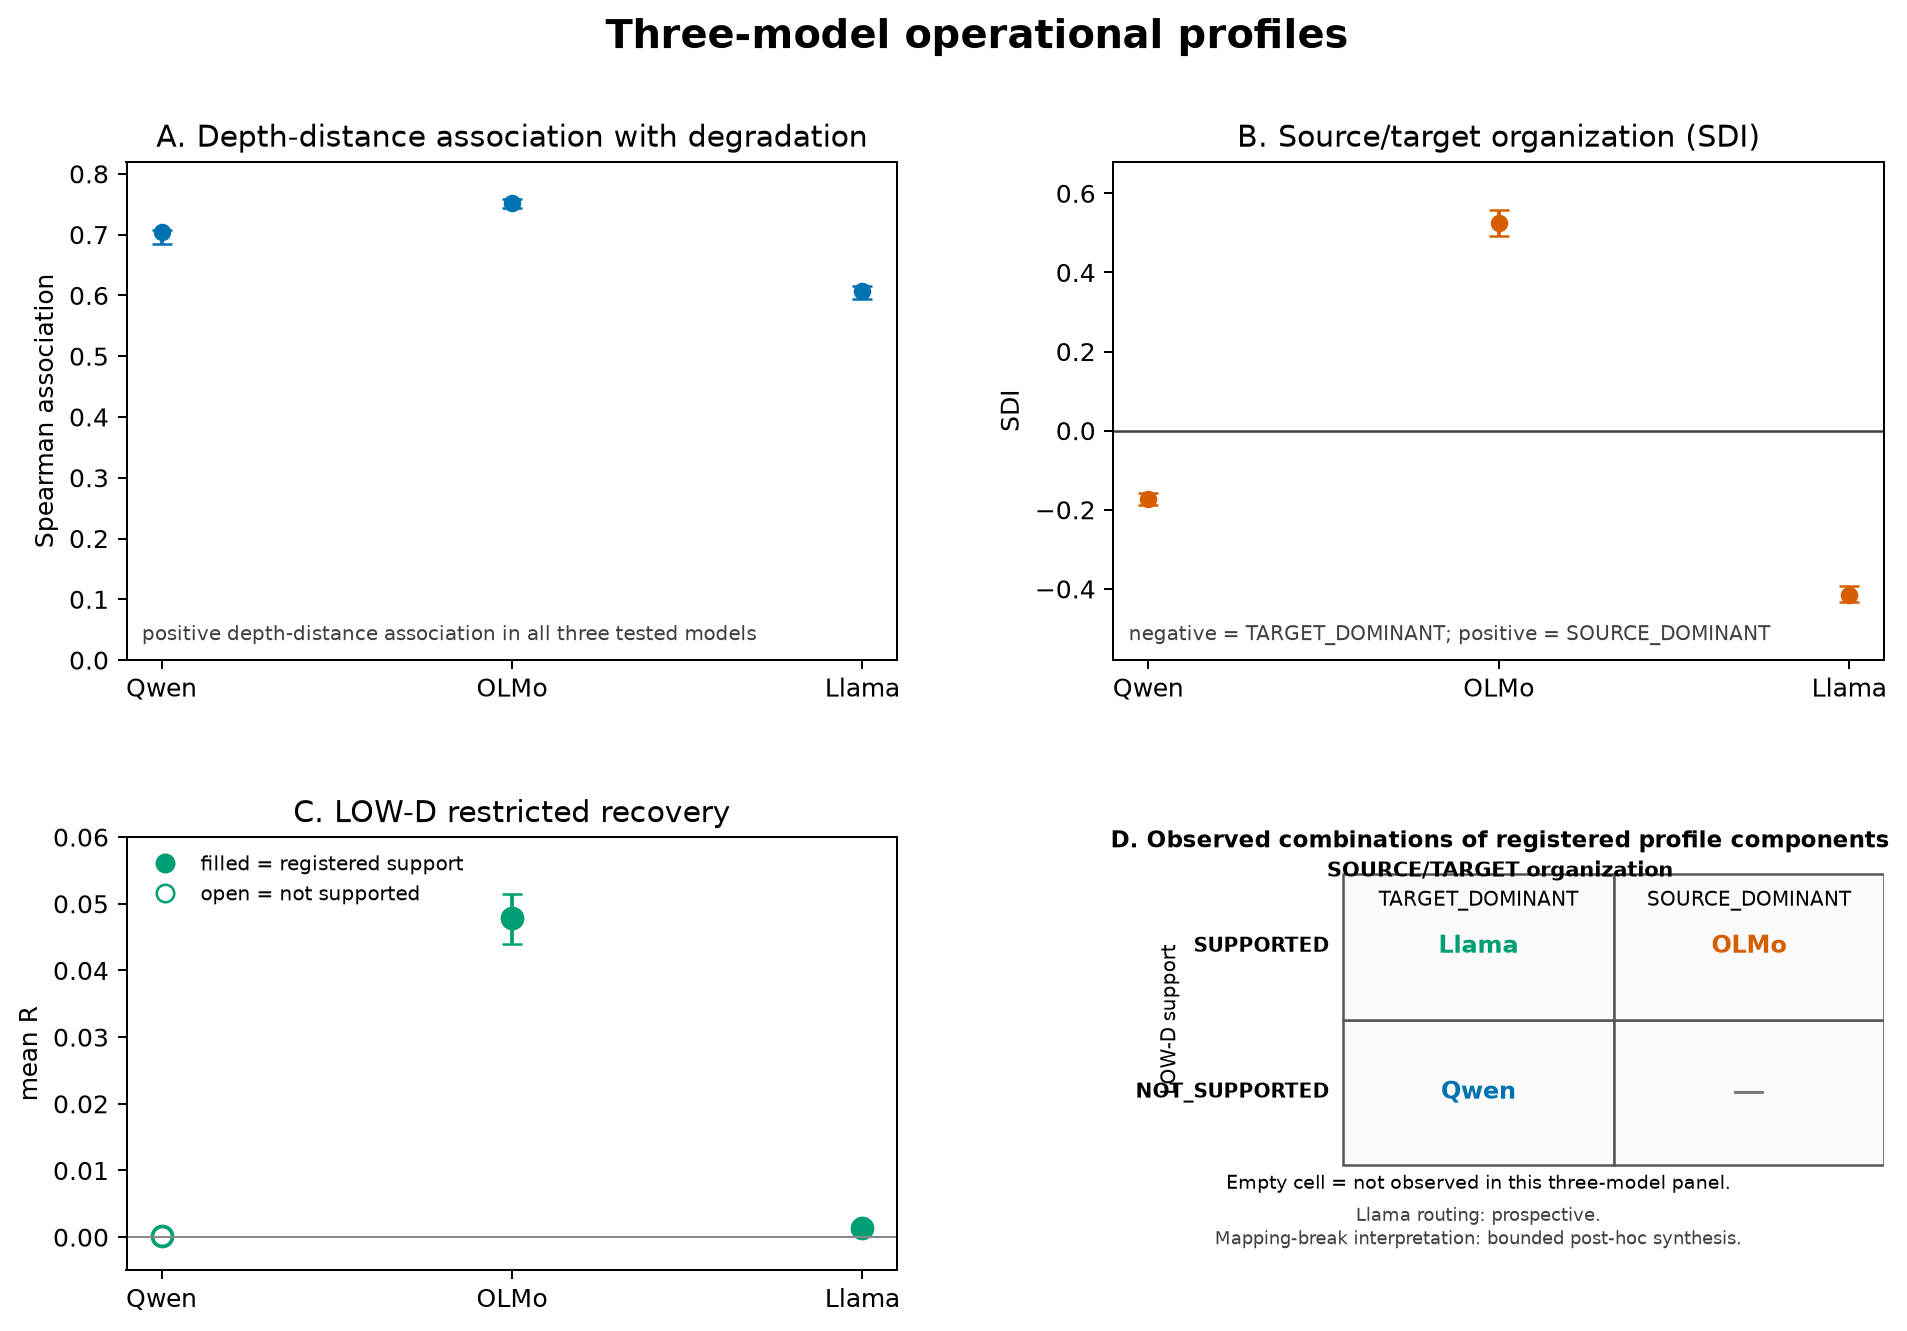
\includegraphics[width=\linewidth]{fig02.png}
\caption{Registered distance association, source/target organization, and LOW-D recovery. Llama routing was prospective; the mapping-break interpretation is bounded post-hoc synthesis.}
\label{fig:profiles}
\end{figure}

Qwen and Llama are target-dominant, whereas OLMo is source-dominant. This is a comparison of organization in the measured matrices; it does not identify why the models differ.

\begin{figure}[t]
\centering
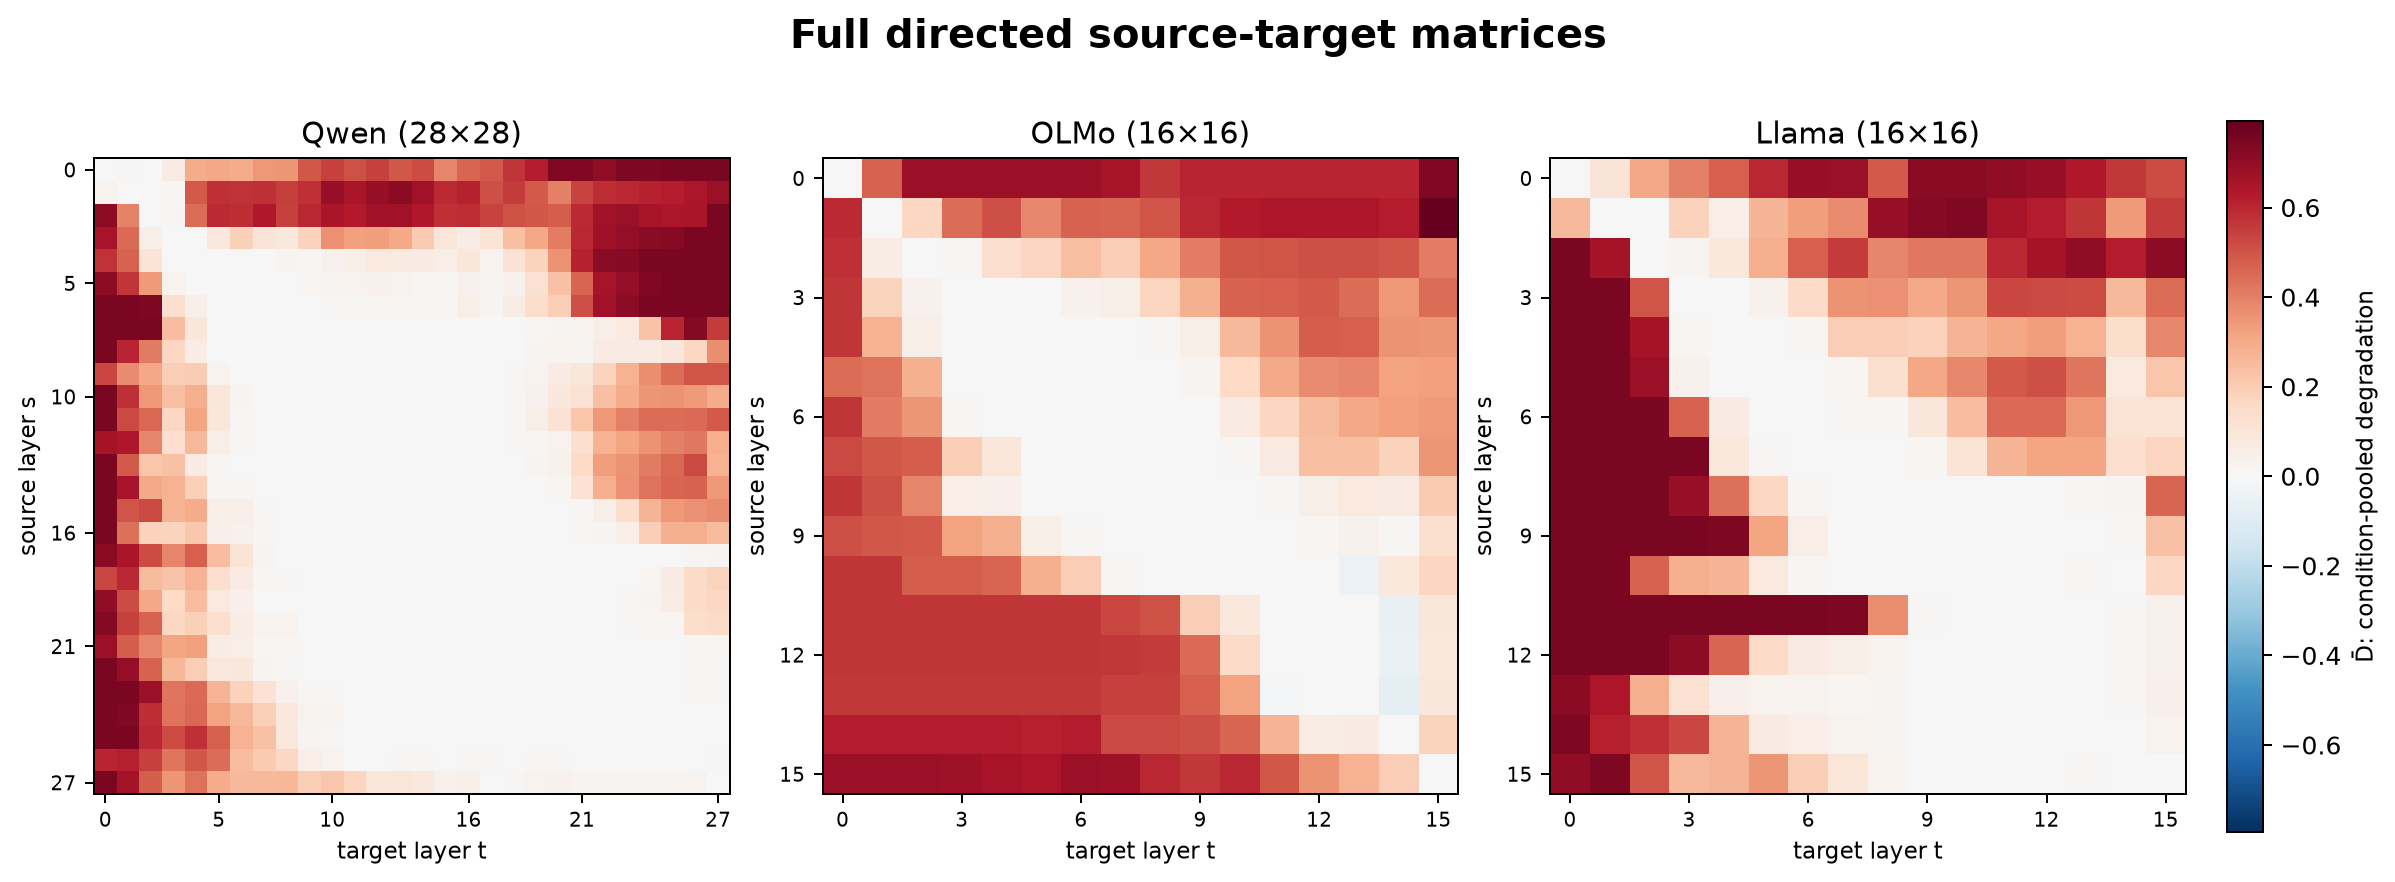
\includegraphics[width=\linewidth]{fig03.png}
\caption{Native-resolution condition-pooled degradation matrices, with source-readout layers on rows and target-representation layers on columns. Orientation is operational. Cross-direction asymmetry is exploratory and does not establish mechanism, causal direction, or any stronger representation claim. Figure 3 visualizes the condition-pooled degradation matrices; the complete C0/D/R matrix artifacts are available through the supplement and machine-readable supplementary artifact.}
\label{fig:matrices}
\end{figure}

\subsection{Restricted LOW-D recovery}
The LOW-D values and bounds are included in Table~\ref{tab:profile}. The Qwen interval crosses zero, while the OLMo and Llama intervals are positive under the registered LOW-D rule. The support labels do not imply equal gain magnitudes or that most selected pairs have positive recovery. The post-closure construct-sensitivity audit further shows that Qwen and Llama LOW-D sets operate near the balanced-accuracy ceiling, whereas OLMo retains substantially more available headroom. Absolute cross-model $R$ magnitudes should therefore not be read as a normalized recovery-capacity scale. Values are rounded for presentation; exact canonical values and the distinction between evaluability and support are in the supplement.

\subsection{Prospective Llama routing and the joint profile}
The initial two-model comparison contained Qwen target-dominant with unsupported LOW-D recovery and OLMo source-dominant with supported LOW-D recovery. Llama was routed prospectively before its result was exposed. Llama exhibits a combination not present in the initial two-model comparison: target-dominant organization together with supported LOW-D recovery. This breaks the simple descriptive mapping suggested by the initial two tested models. The interpretation is a bounded post-hoc synthesis, not a claim of independent dimensions or a universal taxonomy.

\begin{table}[t]
\centering
\caption{Evidence and claim hierarchy.}
\begin{tabular}{p{.22\linewidth}p{.70\linewidth}}
\toprule
Evidence & Bounded claim\\
\midrule
Positive shared structure & Distance-associated degradation appears in all three tested models.\\
Restricted recovery & LOW-D endpoint support differs across models under the registered diagnostic.\\
Source/target organization & Measured source/target organization differs across models.\\
Negative evidence & Complementary-split non-replication and unsupported scalar prediction bound uniform recovery accounts.\\
Prospective triangulation & Llama was routed prospectively; the mapping-break interpretation is bounded post-hoc synthesis.\\
Secondary similarity & Symmetric CKA provides descriptive association with completed operational measurements.\\
Not established & Cross-task robustness, semantic equivalence, information preservation, geometry, mechanism, information flow, causality, and behavioral consequence remain not established.\\
\bottomrule
\end{tabular}
\end{table}

The common distance-associated result coexists with different measured organization and restricted-recalibration profiles. No single scalar score captures all of these operational properties.

\subsection{Secondary CKA comparison}
CKA was added only after core science closure to compare a symmetric representation-similarity measure with completed operational measurements, not to redefine them. On the EVAL split, CKA was positively associated with \texttt{C0} in Qwen (0.8372), OLMo (0.7589), and Llama (0.7706), and negatively associated with \texttt{D} and \texttt{R} in the three models; these are secondary comparisons. Because CKA is symmetric, it remains complementary to rather than a replacement for the directed source-target analysis; full values and pair definitions are in Supplement S3.

\section{Discussion}
\subsection{Direct reuse and restricted recalibratability}
$C0$ asks whether a readout trained at one depth can be used at another without retraining. $R$ asks whether one specific FIT-only calibration improves the target measurement. Restricted recovery was designed as a diagnostic of limited recalibratability, not an attempt to learn the best possible cross-depth transformation. The branch is not zero-shot: its permitted featurewise statistics use target-depth FIT representations, while EVAL labels and outcomes remain excluded. A stronger adapter would answer a different question. Direct failure and restricted recovery should therefore remain separate in reporting.

\subsection{What the three-model comparison adds}
All three models show positive distance-associated degradation, while source/target organization and LOW-D endpoints differ. The common distance relationship coexists with different operational profiles in the tested panel. This is bounded evidence of heterogeneity, not a population-level law, explanation of model differences, or intrinsic model classification.

\subsection{Failure and similarity boundaries}
Failure of a frozen source readout identifies an operational interface mismatch under that readout, not the absence of every task-relevant signal at the target depth. Recovery under one restricted procedure does not establish source-target equivalence, and failure of that procedure does not establish that task-related signal is absent. Directional asymmetry is descriptive and secondary. CKA provides symmetric similarity context; its association with $C0$, $D$, and $R$ does not establish causality, mechanism, information flow, geometry, or equivalence.

\section{Limitations}
The study covers three decoder-only models, one registered carrier, one task panel, and ten surface conditions. The matrices measure operational scores, not all task-relevant information. Restricted recalibration is one low-capacity FIT-only diagnostic and LOW-D depends on its frozen DIAGNOSTIC mask. Headroom differs across models, so absolute $R$ magnitudes are not a normalized recovery scale. Directionality and CKA are secondary, and the conclusions do not generalize beyond the tested conditions without further evidence. Cross-task and task-panel robustness remains NOT\_ESTABLISHED. The prospective EXT-B extension terminated at its frozen dataset-construction gate before model inference and produced no model-level cross-task result; this termination is not a scientific nonreplication.

\section{Conclusion}
Across three tested models, fixed-readout compatibility shows a shared positive distance-associated structure but non-identical source/target organization and restricted-recalibration profiles. Registered negative and non-replication evidence limits a uniform calibration interpretation. The secondary CKA comparison supplies descriptive context without replacing the directed operational measurement. We therefore report a scoped direct-reuse/restricted-recalibration decomposition and a three-model characterization, with claims limited to the tested carrier, panel, models, and conditions.

\section*{Reproducibility Statement}
The methods, registered definitions, split structure, carrier, model identities, conversion provenance, and resampling rule are given in Sections 3 and 4 and the anonymous artifact. The anonymous artifact contains machine-readable matrices, configuration records, exact supplementary values, sanitized model/conversion provenance, and validation metadata. The supplement records the complete canonical profile and secondary comparison. No local filesystem paths or private repository metadata are required for reproduction.

\section*{AI Use Statement}
Generative AI assistance was used for ideation and hypothesis refinement, experimental and method-design feedback, code assistance, result interpretation, literature discovery and summarization, and manuscript organization and drafting. Human authors reviewed the resulting text, citations, claims, and artifacts and remain responsible for the final submission.

\bibliography{references}
\bibliographystyle{iclr2027_conference}

\appendix
\section{Additional Experimental Details}
\label{app:details}

This supplement preserves the epistemic role of the complementary negative evidence and provides compact details for the secondary CKA analysis and the post-closure construct-sensitivity audit. It is not a chronological archive of every project experiment. All claims remain bounded to the registered models, carrier, task panel, splits, and conditions.

\subsection{Complementary-split recovery}
EXP-023 was a registered version-controlled replication of the restricted-recovery question under a complementary split. Split A shows recovery under the registered endpoint, whereas Split B does not. The registered cross-split outcome is \texttt{NO\_REPLICATION}.

This result is evidence of split heterogeneity. It does not show that recovery is absent in every setting, and it is not relabeled as a partial replication by pooling the two splits. Recalibration is an operational diagnostic here, not a mechanism claim.

\begin{figure}[h]
\centering
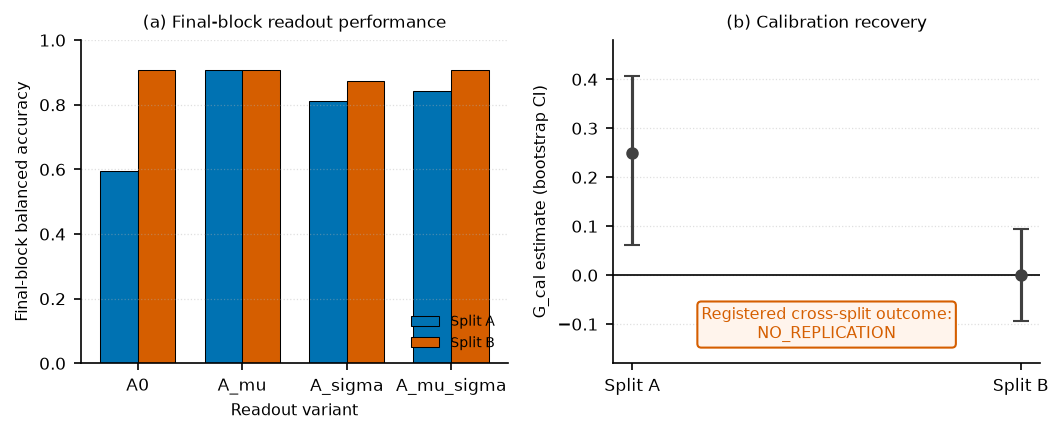
\includegraphics[width=.82\linewidth]{../appendix/figures/fig04.png}
\caption{EXP-023 complementary-split result. Split A supports the registered recovery endpoint and Split B does not; the registered outcome is \texttt{NO\_REPLICATION}. The figure reports the existing validated asset and does not imply uniform recovery or its absence everywhere.}
\end{figure}

\subsection{Registered degradation-based predictor}
EXP-024 tested the registered diagnostic predictor using all 10 registered conditions. The diagnostic is $S_{\mathrm{diag}}(c)$ and the outcome is $G_{\mathrm{eval}}(c)$. The registered association was Spearman $\rho=0.28401877872187725$, with exact one-sided $p=0.2115079365079365$; the registered outcome was \texttt{NOT\_SUPPORTED}.

No post-hoc subset, positivity inference, trend-significance claim, or power-adjusted rescue is introduced. The result limits the interpretation of a single degradation-based scalar predictor; it does not show that no relationship exists under any other measurement or design.

\begin{figure}[h]
\centering
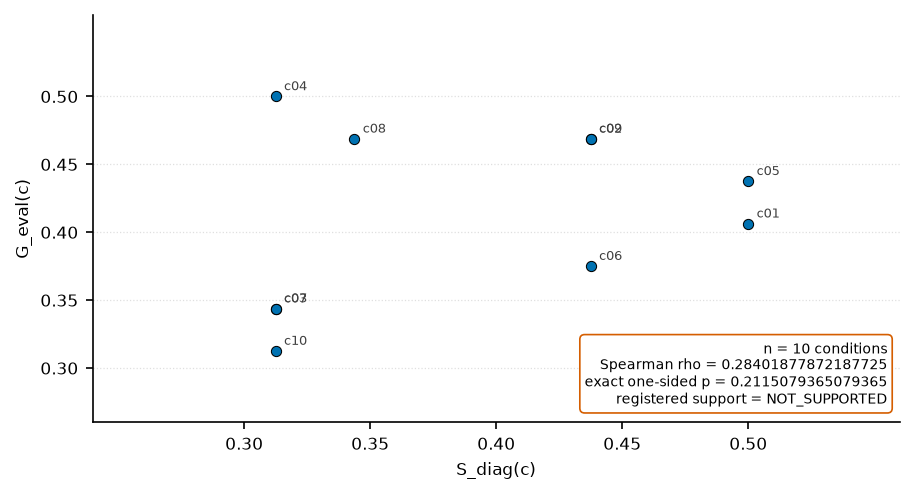
\includegraphics[width=.82\linewidth]{../appendix/figures/fig05.png}
\caption{EXP-024 registered predictor test across all 10 conditions. The plotted diagnostic is $S_{\mathrm{diag}}(c)$ and the outcome is $G_{\mathrm{eval}}(c)$; the exact one-sided test gives $\rho=0.28401877872187725$ and $p=0.2115079365079365$, with registered outcome \texttt{NOT\_SUPPORTED}.}
\end{figure}

\subsection{Secondary CKA comparison}
CKA uses the EVAL split, 640 samples per model, the post-block residual carrier before final normalization, and centered linear CKA. The table reports model-wise off-diagonal Spearman associations; models are not pooled.

\begin{table}[h]
\caption{Secondary CKA associations.}
\centering
\begin{tabular}{lrrr}
\toprule
Model & CKA vs. $C0$ & CKA vs. $D$ & CKA vs. $R$\\
\midrule
Qwen & 0.8372 & -0.8373 & -0.6738\\
OLMo & 0.7589 & -0.8082 & -0.3729\\
Llama & 0.7706 & -0.7634 & -0.5189\\
\bottomrule
\end{tabular}
\end{table}

These are descriptive associations and comparisons with completed operational measurements. CKA is symmetric by construction and does not establish causality, mechanism, information flow, geometry, or equivalence.

\subsection{Post-closure construct-sensitivity audit}
This audit is \texttt{POST\_CLOSURE\_DESCRIPTIVE\_SENSITIVITY}, not confirmatory evidence. Module A exposes the already registered SDI components. Module B0 exposes the already registered LOW-D auxiliaries. Module B1 reports the new, descriptive EVAL headroom summary using the exact DIAGNOSTIC-defined LOW-D mask. The mask is eligible source rows, off-diagonal pairs, and $D^{\mathrm{DIAG}}(i,j)\leq0$; DIAG denotes the DIAGNOSTIC split, not a matrix diagonal, and the mask is not selected from EVAL.

\begin{table}[h]
\caption{Exact canonical three-model profile values and displayed bootstrap bounds.}
\centering
\scriptsize
\resizebox{\linewidth}{!}{%
\begin{tabular}{lrrrrrrrrrrrrrrrr}
\toprule
Model & Distance association & Distance 5\% & Distance 95\% & Distance status & SDI & SDI 5\% & SDI 95\% & SDI class & LOW-D mean & LOW-D 5\% & LOW-D 95\% & Selected pairs & Positive-R fraction & Evaluability & LOW-D support\\
\midrule
Qwen3-1.7B & 0.7049462572 & 0.6851830381 & 0.7080622075 & POSITIVE\_SUPPORTED & -0.1735535241 & -0.1886852743 & -0.1582748746 & TARGET\_DOMINANT & 0.0001392327 & -0.0000993316 & 0.0003610766 & 202 & 0.0742574257 & EVALUABLE & NOT\_SUPPORTED\\
OLMo-2-1B-Instruct & 0.7519250368 & 0.7438987161 & 0.7582397801 & POSITIVE\_SUPPORTED & 0.5249651786 & 0.4910149189 & 0.5584696075 & SOURCE\_DOMINANT & 0.0478571431 & 0.0440289896 & 0.0515186089 & 35 & 0.8285714286 & EVALUABLE & SUPPORTED\\
Meta-Llama-3.2-1B-Instruct & 0.6077483253 & 0.5949008758 & 0.6154160155 & POSITIVE\_SUPPORTED & -0.4142642299 & -0.4342173412 & -0.3923962803 & TARGET\_DOMINANT & 0.0014030612 & 0.0007325690 & 0.0021867916 & 49 & 0.3265306122 & EVALUABLE & SUPPORTED\\
\bottomrule
\end{tabular}}
\end{table}

The corresponding registered support labels are positive-supported distance association for all three models; Qwen LOW-D is \texttt{NOT\_SUPPORTED}, while OLMo and Llama LOW-D are \texttt{SUPPORTED}. Qwen, OLMo, and Llama positive-$R$ fractions are 0.0742574257, 0.8285714286, and 0.3265306122, respectively. The selected-pair counts and interval convention are registered quantities, not majority-vote or normalized-capacity measures.

\subsection{Registered conditions and split boundary}
The ten conditions vary lexical realization, syntactic structure, compression/elaboration, relation explicitness, formal/informal register, a neutral distractor prefix, and anaphoric reference while retaining the registered semantic-class identity. The source-family split prevents related surface conditions from crossing FIT, DIAGNOSTIC, and EVAL. The source readout is fit on FIT only; the restricted calibration may use target-depth FIT representations for its registered featurewise statistics. EVAL labels and outcomes cannot change coefficients, calibration, or pair membership.

\subsection{Artifact and reproducibility index}
The primary result authorities are the version-controlled EXP-022A, EXP-023, EXP-024, EXP-025, EXP-026, and EXP-027 result artifacts, together with the scientific asset register and relevant version-controlled protocol artifacts. The main manuscript records the carrier, source/target indexing convention, classifier and calibration settings, split structure, bootstrap unit, and registered thresholds. Exact hashes and artifact paths are available through the anonymous artifact package.

The full condition-pooled C0, D, and R matrices are available through the machine-readable supplementary artifact and are summarized visually only for D in the main manuscript. The EXP-025 route remains part of the main-text evidence chain: the tested OLMo panel records cross-model heterogeneity in the degradation/recovery profile while its separate degradation-based predictor remains unsupported. No new EXP-025 visualization is introduced in this supplement.

\subsection{Claim boundary}
These materials support statements about measured direct fixed-readout compatibility, degradation, restricted recalibratability under the registered operator, model-dependent profiles, and descriptive association with a secondary symmetric similarity measure. They do not support causal, mechanistic, information-flow, geometric, universal, or deployment claims.

\end{document}
